


%======================================================== %
\subsection*{Question 2}
The masses of 30 human males and 30 arabian stallions were observed. Their masses (in lbs) are given below
{
	\large
	\begin{framed}
		\begin{verbatim}
		Humans
		
		106, 120, 130, 138, 145, 151, 156, 161, 166, 171
		176, 180, 185, 189, 194, 198, 203, 208, 212, 217
		223, 228, 234, 240, 247, 255, 264, 276, 290, 313
		\end{verbatim}
	\end{framed}
}
\newpage
{
	\large
	\begin{framed}
		\begin{verbatim}
		Stallions
		
		808, 824, 835, 843, 851, 857, 862, 868, 872, 877
		881, 886, 890, 894, 898, 902, 906, 910, 914, 919
		923, 928, 932, 938, 943, 949, 957, 965, 976, 992
		\end{verbatim}
	\end{framed}
}
\begin{description}
	\item[a)]	Draw histograms for these samples and compare them with respect to shape, centrality and relative dispersion. 
	\item[b)]	Calculate the medians of these samples (from the raw data).
	
\end{description}
%======================================================== %
\subsection*{Question 3}
\textit{(MA4102 Exam Question from 2011)}

\[\mbox{Image: Week3Boxplotquestion}\]
%\begin{figure}[h!]
%	\centering
%	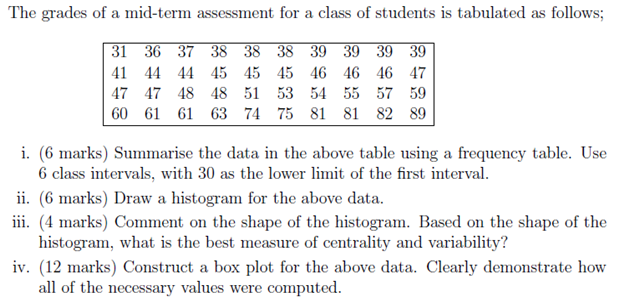
\includegraphics[width=0.9\linewidth]{Week3Boxplotquestion}
%\end{figure}

\subsection{Boxplots}
\begin{center}
	\begin{tabular}{cccccccccc}
		\hline 
		4 & 6 & 8 & 9 & 17 & 17 & 18 & 19 & 20 & 22 \\ 
		
		22 & 27 & 28 & 29 & 31 & 35 & 38 & 39 & 40 & 46 \\ 	
		48 & 56 & 56 & 57 & 57 & 58 & 58 & 60 & 61 & 62 \\ 	
		64 & 66 & 68 & 69 & 74 & 75 & 78 & 79 & 80 & 82 \\ \hline
		
	\end{tabular} 
\end{center}


lower fence?
Upper fence?

Any values above or below fences?






\end{document} 
